\chapter{ACTS starting configuration}

The ACTS consists of at least one UAV, required as the payload needs to be lifted from the ground, and one UGV, included for safety and operational constraints. To fully control the payload in space, we need at least six cables

\section{Connections to the payload}

The configuration of the UAV connections is crucial as it directly affects how forces are applied to the payload.
UAVs are responsible for generating the lifting force required to lift the payload. Consequently, the number of UAVs depends strongly on the payload mass. However, increasing the number of UAVs leads to higher power consumption and greater system complexity. So, adding more UAVs does not necessarily improve performance. 
Additionally, each UAV can be connected to the payload using either a single cable or multiple cables. The choice of configuration affects controllability, wrench feasibility, robustness, and energy efficiency, and should be evaluated accordingly. A practical compromise is to use three UAVs connected to the payload at distinct attachment points, providing a balance between the metrics just mentioned (Figure \ref{fig:uav-possible-configuration}). \\

\begin{figure}
    \centering
    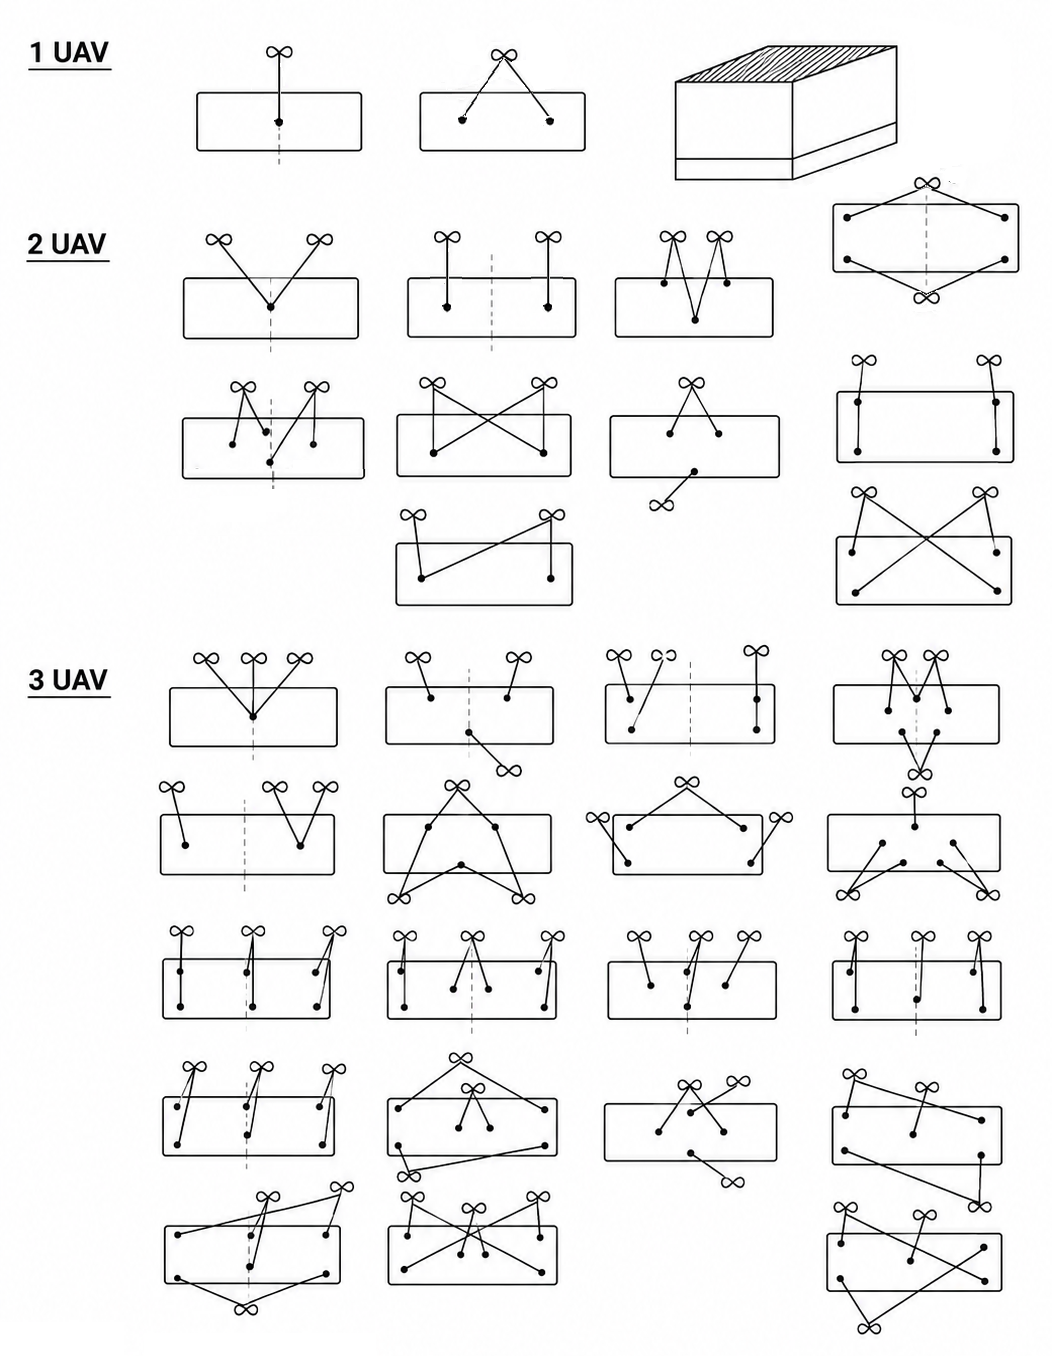
\includegraphics[width=0.58\linewidth]{images/uav_config.png}
    \caption{Possible UAVs connection to the payload}
    \label{fig:uav-possible-configuration}
\end{figure}

\todo[inline]{Not actually this the reason: especially in ourcase the hook are fixed in space so they are independent, look to what said for the ppt}
In contrast, UGVs do not contribute to lifting the payload, and therefore do not require multiple cable connections for stability. In most cases, a single cable connection between each UGV and the payload is sufficient. Adding more cables would increase system complexity without significant benefits. Since the system is designed to be redundant, the overall number of UAVs and UGVs must be carefully selected.

\begin{figure}
    \centering
    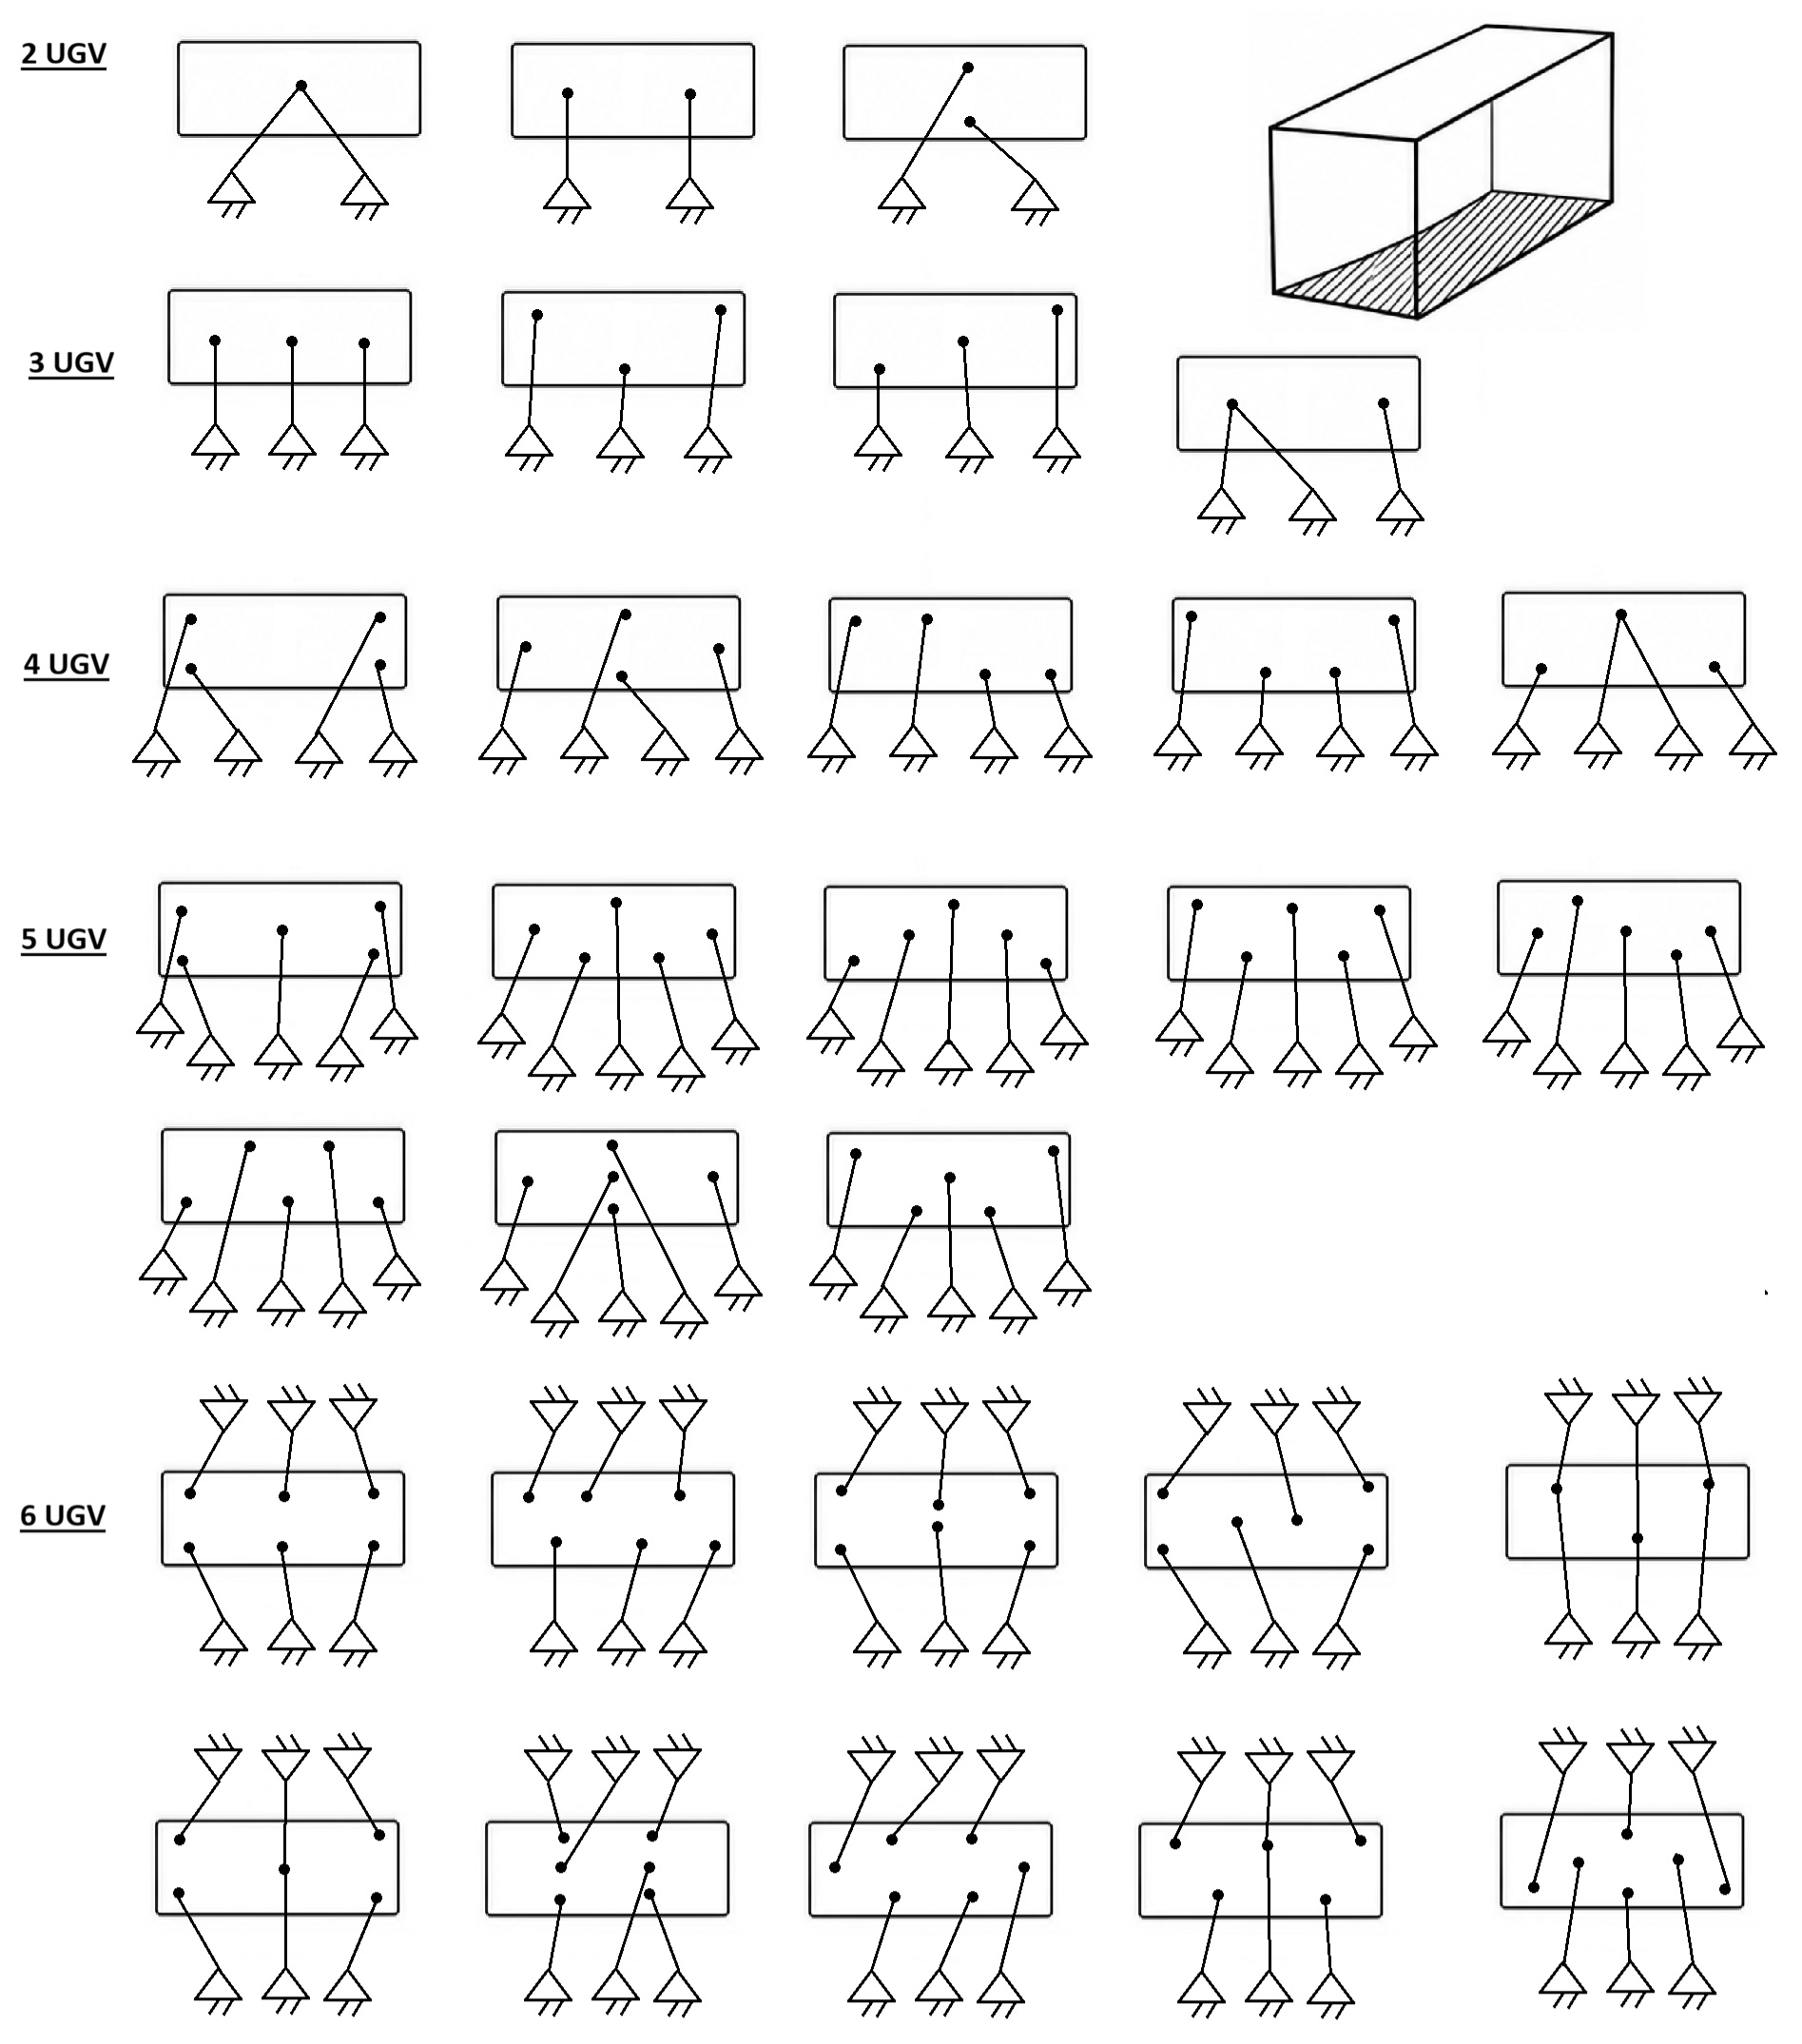
\includegraphics[width=0.58\linewidth]{images/ugv_config.jpeg}
    \caption{Possible UGVs connection to the payload}
    \label{fig:UGV_configuration}
\end{figure}

\section{Force Control on point-mass payload}
Before going into details on the full consideration, let's analyze some simpler configurations.

\subsection{Case: one drone connected to the ground through a cable}
\label{sec:forceControl1droneToGround}
The goal is to design the drone force $F_{prop}$ such as that the ground tension is controlled. Since only a tension in the cable direction is imposable, an arbitrary force $f^*$ at the ground anchor can be achieved only by moving the drone, changing the cable direction $u$. Called $a$ the drone's position and $b$ the attachment point to the ground:
  \begin{equation}
    u = \frac{a-b}{\|a-b\|}
  \end{equation}

\begin{figure}[ht]
    \centering
    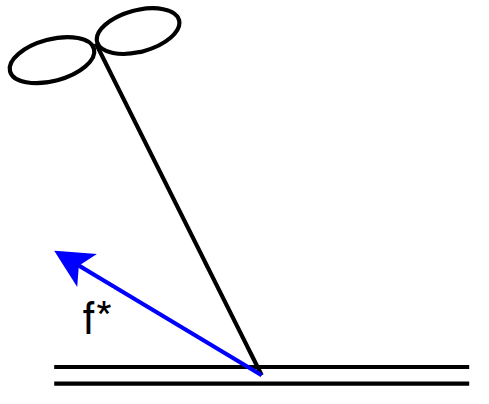
\includegraphics[width=0.3\linewidth]{images/1drone1cableGroundAnchor.png}
    \caption{One drone system connected to the ground through a cable}
    \label{fig:1drone1cableGroundAnchor}
\end{figure}

\subsubsection{Option 1}
Defined the desired cable tension $\tau^*$ and the desired cable direction $u^*$ as:

\begin{minipage}[t]{0.45\textwidth}
  \begin{equation}
    \tau^* = \|f^*\|
    \label{eq:tau_des}
  \end{equation}
\end{minipage}\hfill
\begin{minipage}[t]{0.45\textwidth}
  \begin{equation} 
    u^* = \frac{f^*}{\|f^*\|}
    \label{eq:u_des}
  \end{equation} 
\end{minipage}

\noindent the ground tension is obtained using the geometric constraint which relates the anchor point to the drone position:
\begin{equation}
    a^* = b + l \, u^*
    \label{eq:geometricContraintOnUAV}
\end{equation}
where $l$ is the cable length. Equation \ref{eq:geometricContraintOnUAV} is then used as a reference to compute the propeller force.
\begin{equation}
    F_{prop} =  m_i g e_3 + K_p (a^*-a) + K_d (\dot{a}^* - \dot{a}) + \tau^* u
\end{equation}

\subsubsection{Option 2}
Given the drone Newton's Second Law described in Equation \ref{eq:uavbalance}, we are able to estimate the cable force $\hat{f} = F_{a, i}^{est}$
\begin{equation}
    m_i \ddot{a}_i = F_{prop, i} - \hat{f} + F_{g, i} \qquad \xrightarrow[]{} \qquad \hat{f} = F_{prop, i} + F_{g, i} - m_i \ddot{a}_i
    \label{eq:uavNewton2law}
\end{equation}
where all the forces are in the world frame and $\ddot{a}_i$ is the drone linear acceleration. Using Equation \ref{eq:uavbalance}, we would like to apply a propulsion force equal to 

\begin{equation}    
    F_{prop, i}^* = f^* - F_{g, i}
\end{equation}
Finally, the closed loop equation is:

\begin{equation}
    F_{prop, i} = F_{prop, i}^* + K_p e + K_d \dot{e}
    , \quad \text{with } e = f^* - \hat{f}
\end{equation}
The result is given to the attitude controller, which aligns the body z-axis with the commanded thrust vector.

\subsection{Case: payload connected to the ground and a drone}
In this case, we are working with the simplified case of an ACTS composed by a drone, a ground anchor and a point-mass payload. Called with subscript 1 the cable that connects the payload to the drone and with 2 the one that connects it to the ground, for definition the vector $u_i$, $i = 1\div n$ is given by 
  \begin{equation}
    u_i = \frac{a_i-p}{\|a_i-p\|}
  \end{equation}
being $a_i$ and $p$ respectively the actuator and the payload position.

\subsubsection{Payload position control}
The goal is to design $F_{prop, 1}$ such that the payload reaches a desired position ($p \xrightarrow{}p^*$), which is reachable for the length of the cable.

\begin{figure}[h]
    \centering
    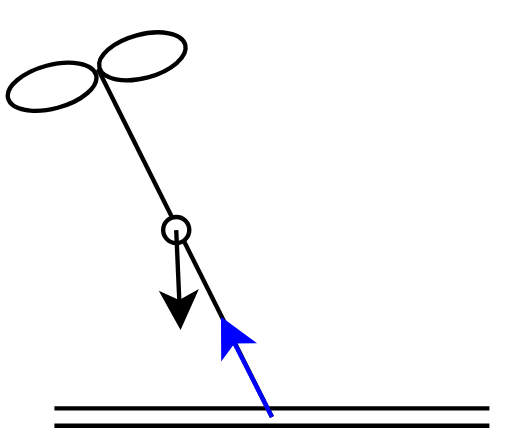
\includegraphics[width=0.3\linewidth]{images/1drone2cablesPayloadGroundAnchorTensionAlongCable.png}
    \caption{Simplified ACTS with one drone and one ground anchor}
    \label{fig:1drone2cablesPayloadGroundAnchorTensionAlongCable}
\end{figure}


The payload dynamics is given by:
\begin{equation}
\begin{aligned}
    m_p \ddot{p} &= \tau_1 u_1 + \tau_2 u_2 - m_p g e_3 \\
    &= F_{a, 1} + F_{a, 2} + F_g \\
    &= F_p + F_g \\
\end{aligned} \quad \xrightarrow[]{}\quad  F_p =m_p (\ddot{p} + ge_3)
\label{eq:Fpdynamics}
\end{equation}
The desired payload force is defined using an impedance controller:
\begin{equation}
    F_p^* = m_p (\ddot{p}^* + ge_3) + K_p (p^*-p) + K_d (\dot{p}^* - \dot{p})
\label{eq:impedancePayloadcontrol}
\end{equation}
with $\dot{p}^*=0$ and $\ddot{p} = 0$ as we required the payload to maintain the position once it is reached. 
The remaining force to be generated by cable 1 is:
\begin{equation}
    F_{a,1}^* = F_p^* - F_{a,2}
\end{equation}
where $F_{a, 2} = \tau_2u_2$. This brings us back to the situation in Section \ref{sec:forceControl1droneToGround}, where $F_{a,1}$ is $f^*$.

\subsubsection{Tension and orientation control}
The goal can also be design $F_{prop,1}$ such that an arbitrary force $f^*$ on the ground can be applied ($F_2 \xrightarrow{} f^*$). In other words, $u_2 \xrightarrow{} u_2^*$ and $\tau_2\xrightarrow{}\tau_2^*$. This case can be interesting to study as in a redundancy system situation, it may be helpful to add additional constraint in one of the cables.
The only difference from the previous case is that the desired position for the payload $p^*$ is not an input anymore, but obtained such that the 2nd cable is aligned along the desired direction given by $f^*$ (Equation \ref{eq:tau_des} and \ref{eq:u_des}). Then:
\begin{equation}
    p^* = a_2 - l_2 u^*_2
\end{equation}

\begin{figure}[h]
    \centering
    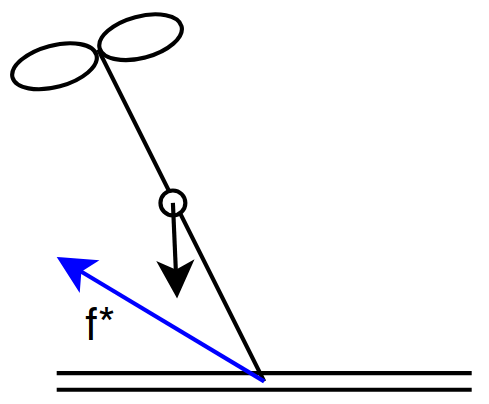
\includegraphics[width=0.25\linewidth]{images/1drone2cablesPayloadGroundAnchor.png}
    \caption{Tension directed arbitrary}
    \label{fig:1drone2cablesPayloadGroundAnchor}
\end{figure}

\subsection{Case: payload connected to the ground through two cables}
The ACTS consists of a point-mass payload connected to the ground through two cables and to an UAV. The enumeration is shown in Figure \ref{fig:1drone2cablesToground}.

\begin{figure}[h]
    \centering
    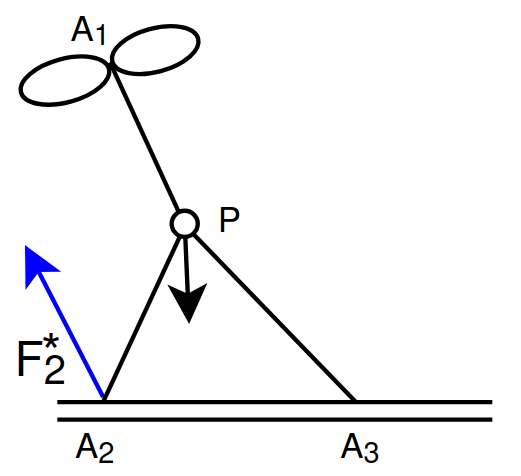
\includegraphics[width=0.3\linewidth]{images/1drone2cablesToground.png}
    \caption{Payload connected through two cable to the ground}
    \label{fig:1drone2cablesToground}
\end{figure}

\subsubsection{Payload position control}
If the input is the desired payload position $p^*$, we find ourselves in three situations:
\begin{enumerate}
    \item $p^*$ lies precisely on the intersecting boundary arcs dictated by the maximum lengths of the ground cables;
    \item $p^*$ is out of reach;
    \item $p^*$ is inside the triangle $A_1A_3P$, resulting into slack cables
\end{enumerate}

In the first case, $p^*$ is used to compute the desired payload force $F_p^*$ (Equation \ref{eq:impedancePayloadcontrol}). Using the simplified payload balance equation related to the forces acting on the payload (Equation \ref{eq:ForceOnPayload}), we obtain the following.
\begin{equation}
    F_{a, 1}^*=F_p^* - \sum_{i=2}^{n} F_{a, i}
\end{equation}
which brings us back to the previous case. 

Because the payload is physically constrained at a boundary where both ground cables are stretched straight, any movement or external disturbance is perfectly resisted by the tension of the cables.

In the second case, since the ground cables physically block the payload from reaching $p^*$, a steady error $e=(p^*-p)\ne 0$ builds up. The actual tension will be directly proportional to the control gains and the distance of the unreachable input:
\begin{equation}
    \sum F_{virtual} \propto (p^* - p_{geom}) \quad \implies \quad \sum F_{virtual} = K (p^* - p_{geom})
\end{equation}
where $p_{geom}$ is the closest reachable point that lies on the workspace boundary. In this case, we may impose a controlled tension on the ground cables directed along $(p^* - p_{geom})$ to ensure the drone continues to pull toward the desired target:

\begin{equation}
    F_{a, 1}^*=F_p^* -\sum_{i=2}^{n} F_{a, i} + F_{virtual}
\end{equation}

In the last case, the distance from the anchors to the payload is less than the cable length, resulting into slack cables as the latter cannot push. Mathematically $\tau_2= 0$ and/or $\tau_3=0$. Then, $F_{a,1}^*= F_p^*$

\subsubsection{Desired tension in the cable on the ground}
The desired variable to control is the tension of one of the cables $F_{a,2} \xrightarrow{} f^*$. 

\begin{equation}
    F_{a, 1}^*=F_p - f^* - F_{a,2}
\end{equation}
where $F_p = m_p (\ddot{p} + ge_3)$ and $F_{a, 2} = \tau_2u_2$.


\subsubsection{Desired tension difference between the cables on the ground}
The desired variable to control a linear combination of the two $F_{a, 2} + \alpha F_{a, 3} \xrightarrow{} f^*$.

\begin{equation}
    F_{a, 1} = F_p - F_{a, 2} - F_{a, 3} 
    \qquad \implies \qquad 
    \begin{aligned}
        F_{a,1}^* &= F_p - (f^* - \alpha F_{a, 3}^* + F_{a, 3}^*) \\
        &= F_p - f^* - (1-\alpha)F_{a, 3}
    \end{aligned}
\end{equation}
For the specific case where $F_{a, 2} - F_{a, 3} \to f^*$:
\begin{equation}
    F_{a,1}^* = F_p - f^* - 2F_{a, 3}^* = F_p - f'^*
\end{equation}


\section{Performance Indices}
\label{sec:performanceIndices}
In the context of the ShieldBot project, we are working with two questions:
\begin{enumerate}
    \item Which attachment geometry gives the best ability to generate the required payload wrench over the entire mission workspace?
    \item Given the chosen architecture, where should the actuators (UAVs and anchor points in the ground) be positioned and what cable lengths should be used during operation?
\end{enumerate}

\noindent In both cases, we need an objective measurement that guides us in the selection. \\

\noindent Every configuration to be eligible needs to satisfy feasibility metrics first, such as \cite{cheng_cable_2023}:
\begin{itemize}
    \item Wrench closure conditions (WCC), which guarantees that the payload is fully constrained and arbitrary wrenches can be generated. Mathematically:
    $
    \text{rank}(J_p) = 6
    $
    and positive tensions exist.
    \item Wrench Feasible Condition (WFC), which checks whether tensions remain in the feasible bound $0\le \tau_{\text{min}} \le \tau \le \tau_{\text{max}}$, included UAV thrust limits, cable strength limits and UGV friction limits in a future where the ground anchor point will be movable.
    \item Interference-Free Condition (IFC), ensuring that there is no cable rubbing and no collision with payload edges. Mathematically:
    \begin{equation}
        \begin{aligned}
            d_{ij} \ge d_{\text{safe}}, \quad &\text{where } d_{ij} = \text{dist} \left(\text{cable } i, \text{cable } j\right) &\forall i, j \\
            d_i \ge d_{safe}, \quad &\text{where } d_i = \min_{s\in [0, 1]} \left( \text{dist} \left(r_i + s(a_i - r_i), P \right) \right) &\forall i 
        \end{aligned}
        \label{eq:IFCconstraint}
    \end{equation}
    where $P$ is the payload geometry and $d_{safe}$ is a clearance threshold.
\end{itemize}

\todo[inline]{check that this is a right conclusion}
However, assuming that all cable attachment points are on the same face of the payload, the only feasible interference between the latter and one of the cables is a near-tangent cable that touches that face. This requirement will be assumed to always be met, as this study places the ACTS in a scenario where this corner case is rarely encountered.

After passing the feasibility filters, we need a way to assign a score to each hook configuration.

\subsubsection{Capacity margin or minimum degree of constraint satisfaction}
The capacity margin is a robustness index that is used to analyze the degree of feasibility of a configuration. It is defined as the shortest signed distance from the task wrench to the boundary of the available wrench set (AWS). Mathematically, it is the minimum of the distances of each one of the $n$ vertex $w_{e, j}$ to each one of the $p$ facet $\left( \mathbf{a}_l, b_l\right)$ of the AWS.
\begin{equation}
    \gamma = \min_{j = 1 \div n} \, \min_{l = 1\div p} \gamma_{j, l}, \quad \text{where } \gamma_{j, l} = \frac{b_l - w_{e, j}^\top \mathbf{a}_l}{\|\mathbf{a}_l\|_2}
\end{equation}
where $\mathbf{a}_l$ is the normal vector to the $l$-th facet and $b_l$ is its offset \cite{pott_arachnis_2015}.

\subsubsection{Worst-Case Capacity Margin}
Additionally, we can define the worst-case capacity margin as how far the system remains from actuator saturation in the most demanding operating condition. Mathematically:
\begin{equation}
    \zeta = \min \left(1 - \max_i \frac{\tau_i}{\tau_{i, max}} \right)
\end{equation}

For each drone, the maximum available cable tension $t_{i, max}$ is based on its maximum thrust $f_{i, max}$ and its current orientation relative to the cable \cite{erskine_wrench_2019}
\begin{equation}
t_{i, max} = m_i \boldsymbol{u}_i^T (\boldsymbol{g} - \ddot{\boldsymbol{x}}_i) + \sqrt{f_{i, max}^2 + m_i^2 \left( \left( \boldsymbol{u}_i^T (\ddot{\boldsymbol{x}}_i - \boldsymbol{g}) \right)^2 - \ddot{\boldsymbol{x}}_i^T \ddot{\boldsymbol{x}}_i - \boldsymbol{g}^T \boldsymbol{g} \right)}
\end{equation}
Considering only quasi-static motion, this can be reduced to the following, where $u_{iz} = \begin{bmatrix} 0 & 0 & 1 \end{bmatrix} \boldsymbol{u}_i$ and $g = \begin{bmatrix} 0 & 0 & 1 \end{bmatrix} \boldsymbol{g}$.
\begin{equation}
    t_{i, max} = m_igu_{iz} + \sqrt{f_{i, max}^2 + m_i^2 g^2 \left(u_{iz}^2 - 1 \right)}
\end{equation}

\subsubsection{Radius of Available Wrench (rAw)}
The radius of the available wrench (rAW) is the maximum magnitude of force that the system can generate uniformly in all directions while remaining within admissible tension limits \cite{jamshidifar_static_2020}. Its optimization helps identify arrangements that simultaneously maximize force robustness, geometric and collision-avoidance constraints, resulting into an enlargement of the static workspace \cite{jamshidifar_static_2020}.

\begin{equation}
    rAW = \min_i \left( \min \left(\frac{|d_{pi}|}{\|\mathbf{n}_{null, i} \|}, \frac{|d_{qi}|}{\|\mathbf{n}_{null, i} \|} \right)\right)
\end{equation}
being $u_{null, i} = \text{null}(M_i)$ with $M_i$ containing combinations of linearly independent cable unit vectors and $d_{pi}$ and $d_{qi}$ defined as:
\begin{equation}
    \begin{aligned}
        d_{pi} &= \sum_{j \in I^+} \tau_{max} u_{nulli}^T u_j + \sum_{j \in I^-} \tau_{min} u_{nulli}^T u_j - m |u_{nulli}^T g| \\
        d_{qi} &= -\sum_{j \in I^-} \tau_{max} u_{nulli}^T u_j - \sum_{j \in I^+} \tau_{min} u_{nulli}^T u_j - m |u_{nulli}^T g|
    \end{aligned}
\end{equation}
However, since \cite{jamshidifar_static_2020} consider the case of a point-mass payload, it does not take in consideration the torques, we may compute separately rAW$_{force}$ and rAW$_{moment}$, the maximum pure force (resp. torque) the platform can exert in any direction while generating zero net moment (resp. linear force).


\subsubsection{Conditioning index}
The conditioning index measures how uniformly the system can generate forces and moments in different directions. Mathematically:
\begin{equation}
    \nu = \frac{\sigma_{\min}(J_p)}{\sigma_{\max}(J_p)} \in [0, 1]
\end{equation}
$\sigma_{\min}$ and $\sigma_{\max}$ are the minimum and maximum singular values of the Jacobian matrix, obtained via Singular Value Decomposition (SVD) \cite{erskine_dynamic_2021}. A small conditioning number indicates a well-conditioned system, far-away from singular configuration.

\subsubsection{Manipulability}
The manipulability index, defined as $w = \sqrt{\text{det}(J_pJ_p^\top)}$, measures the volume of the wrench ellipsoid. A value close to 0 means that the system hit a kinematic singularity, while large value means a large overall wrench generation capability.

\section{Architecture Selection Strategy}
\todo[inline]{Say that this is an option but then just announced which one we used, but it will be talken better in the next chapter}
Once the feasibility constraints are satisfied, we may want to proceed either by
\begin{equation}
    N =w_1 \hat{\gamma} + w_2 \,  \hat{\text{rAw}} + w_3 \hat{\zeta}
\end{equation}
where all the metrics are scaled to $[0, 1]$, or either choosing the solution that maximizes the radius of available wrench between all the solutions that satisfy $\gamma > \gamma_{\text{min}}$ and using the worst-case capacity margin as a tie breaker.

Our solution will finally be:
\begin{equation}
    U^* =\arg \max_U \left(N(U) \right)
\end{equation}

We are interested in working with an over-actuated system. Therefore, we will start using six cables for fully control the payload pose and three drones acting as an anti-gravitational force. A schematic is shown in Figure \ref{fig:6cables3dronesSchem}. 


\begin{figure}[h]
    \centering
    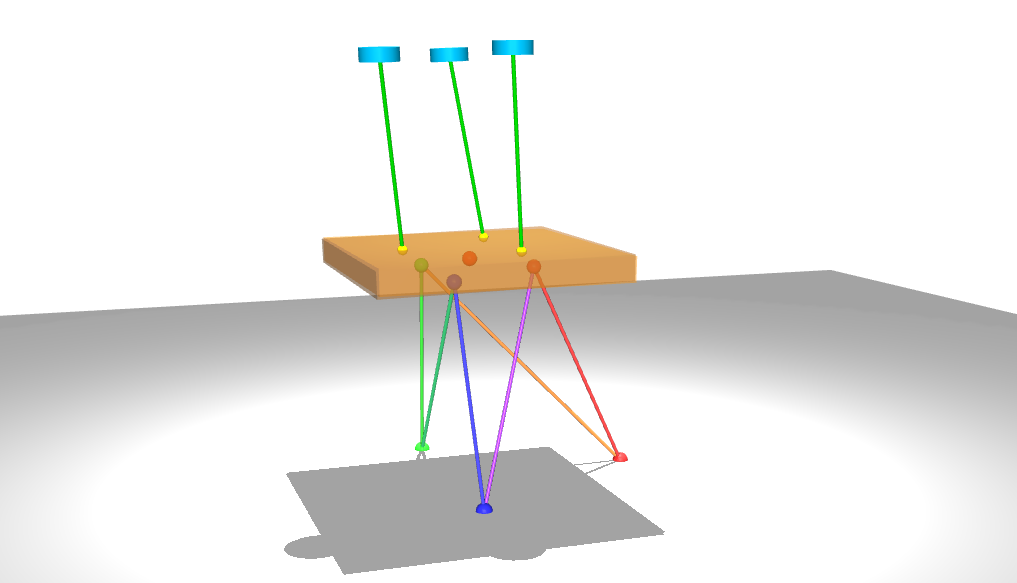
\includegraphics[width=0.8\linewidth]{images/acts_stewart_mujoco.png}
    \caption{Over actuated ACTS with 6 ground cables and 3 UAVs}
    \label{fig:6cables3dronesSchem}
\end{figure}